%----------------------------------------------------------------------------
\chapter{Implementation of the dynamic fraud detection scenario}
%----------------------------------------------------------------------------

This chapter discusses the reactive database setup for each new transaction and how incremental view maintenance can be applied in our static implementation.
In dynamic fraud detection experiments, the Neo4j APOC library is used in the database environment.
For the demo purposes, a web application bundle is developed using popular JavaScript libraries, including Angular and NodeJS.
Finally, the query execution time is benchmarked in comparison with the static implementation. 

%----------------------------------------------------------------------------
\section{Incremental view maintenance}
%----------------------------------------------------------------------------

Graph processing is becoming more challenging with a growing database scale.
A growing real-world database workload is dynamic; higly transaction environment might experience millions of inserts per second.
To execute the active middleware queries at each transaction increases the workload and remains the top priority in database optimization problems.
To eliminate the query to be calculated over the whole database, \emph{incremental view maintenance} techniques can be used0.
To achieve the incremental view maintenance support in our database, we designed the delta queries for different fraud scenarios.
Delta queries are designed to be executed along with each new transaction commit.
The query covers only the required portion of the database (\autoref{fig:incremental_vm}).
In theory, the queries are calculated in relational algebra~\cite{SzarnyasPhD} and turned into delta queries automatically using derivation rules. In our case, we performed the derivation manually using the intuitive meaning of the queries.
Procedures are set up in the Neo4j database engine and triggered transaction events.
In our implementation, we introduce new parameters for nodes, and each transaction procedures assign them.

\begin{figure}[!ht]
  \centering
  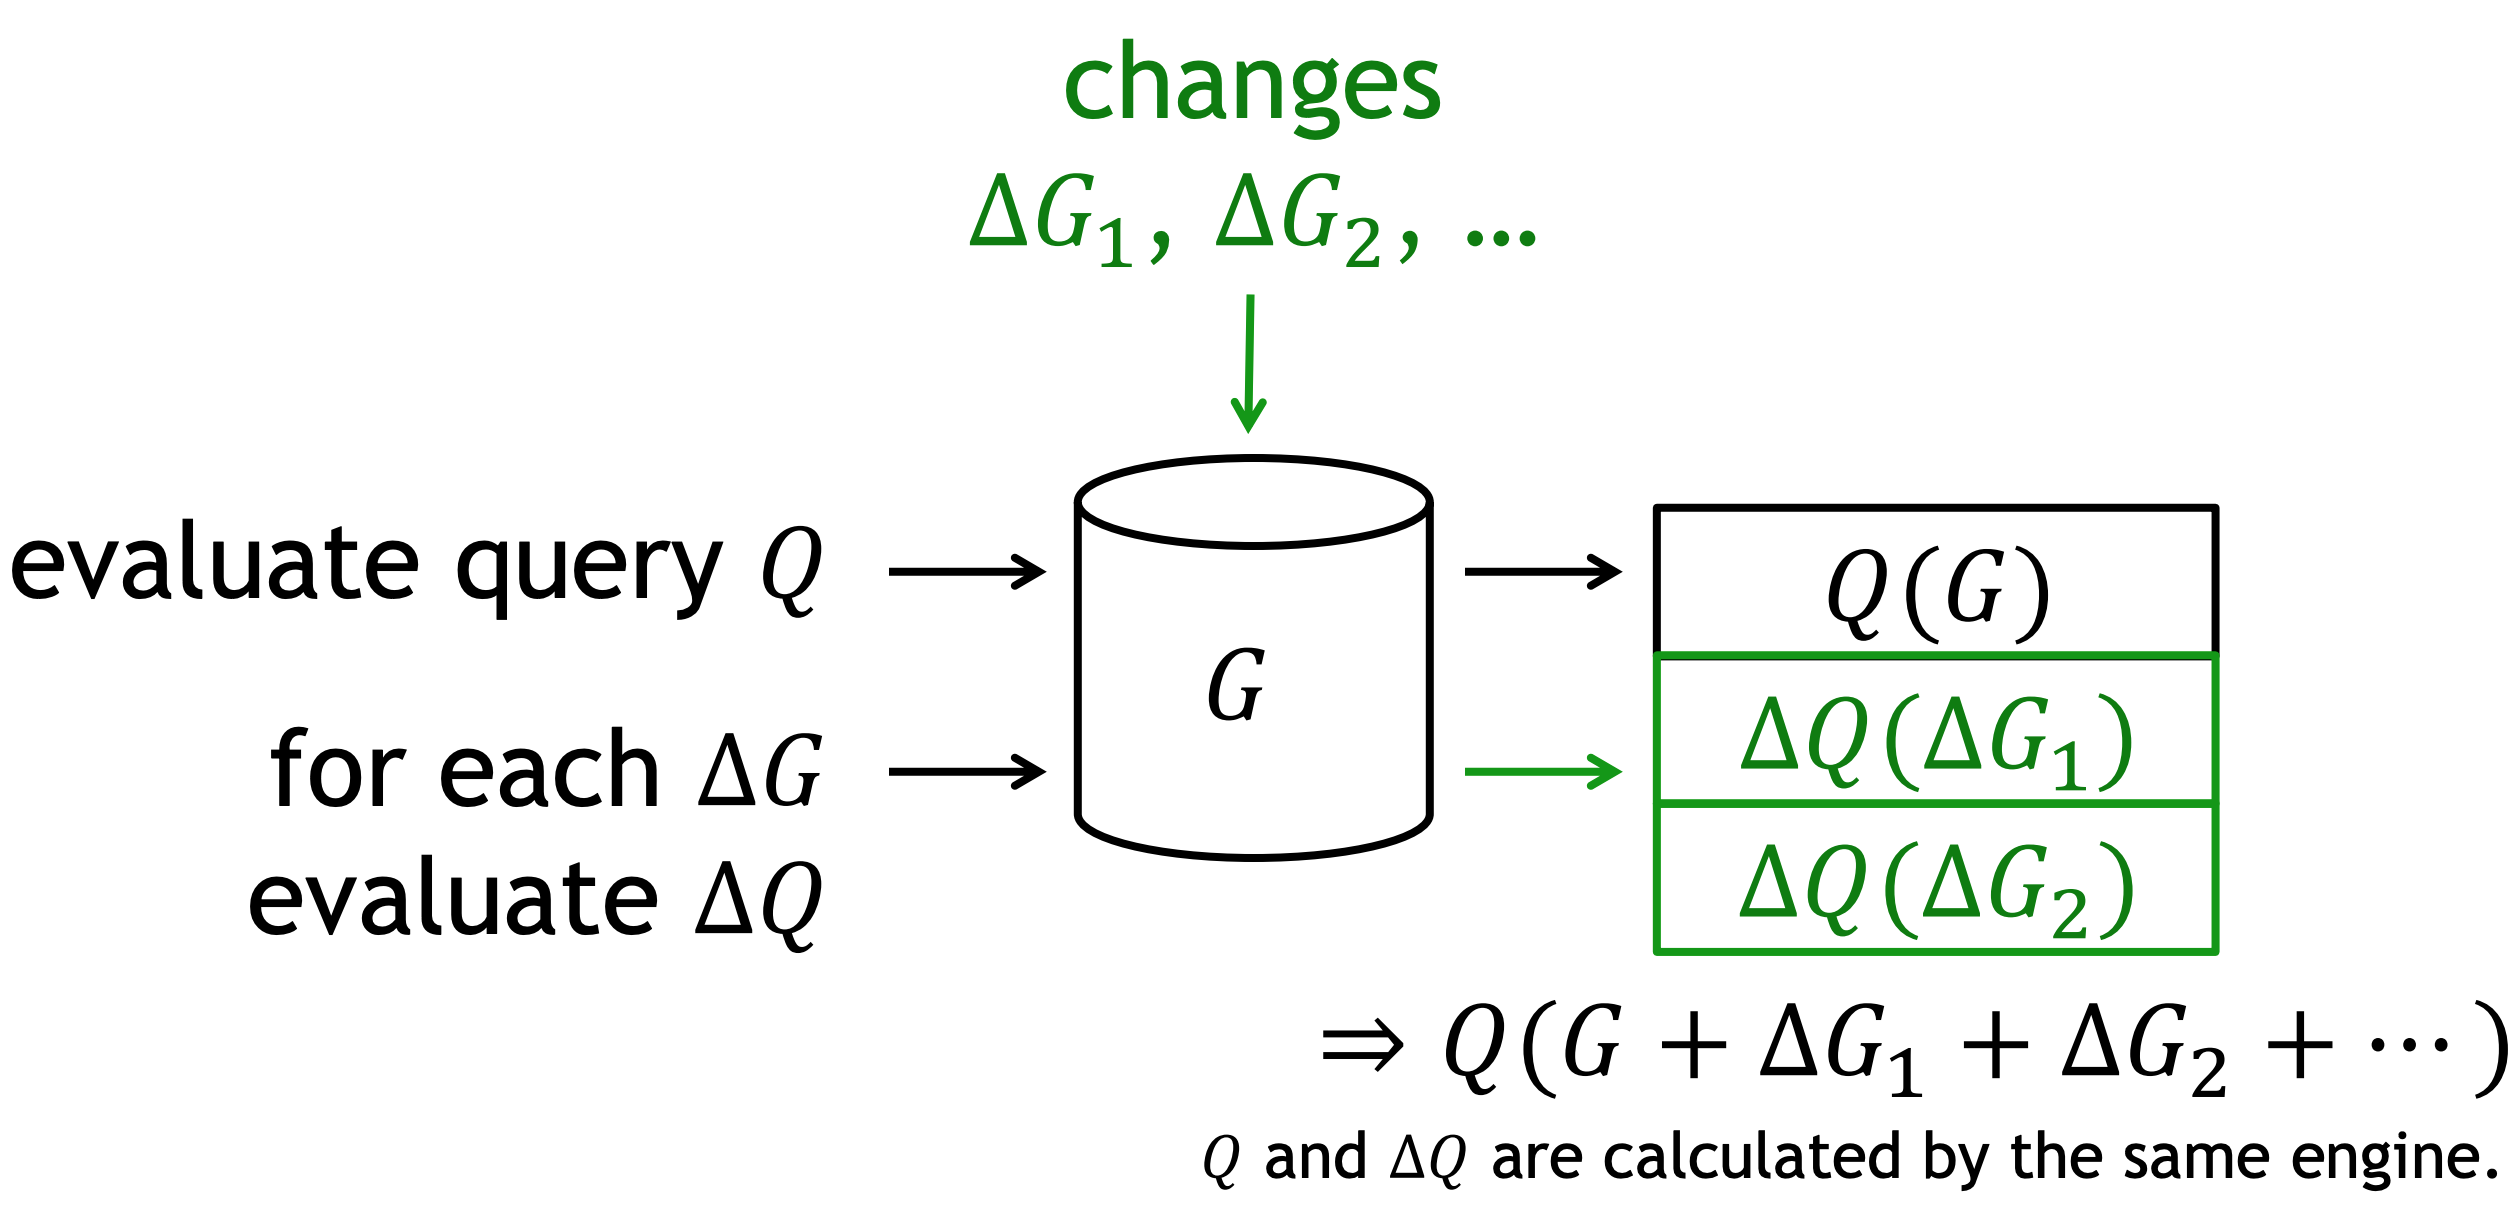
\includegraphics[width=0.8\textwidth]{figures/incremental_view_maintenance.png}
  \caption{Delta queries in databases~\cite{talks/OCIM4/ivm}} 
  \label{fig:incremental_vm}
\end{figure}

%----------------------------------------------------------------------------
\section{Software stack of monitoring platform}
%----------------------------------------------------------------------------

\subsection{General structure}

For demonstration purposes, a web stack software bundle is developed to monitor real-time changes in the graph database.
Users can query the fraud actors, relationships with different categories in the web application, inject the new random fraud data, and get dynamic notification about the recent changes.
The software bundle is a connected four components ecosystem over the internet TCP/IP protocol; web application, local graph database, cloud server, and notification service provider (\autoref{fig:software_stack}).
A single complete detection workflow consists of 5 steps:

\begin{enumerate}
  \item \textbf{Fraud injection} The random fraud relationships are generated in the web application and commit them to the graph database as a new transaction. 
  \item \textbf{Notify cloud server about new changes} The web application notifies the cloud backend about new successful database transactions.
  \item \textbf{Query graph database for updates} The web server will query the graph database and compare the new fraud statistics with its last saved version.
  \item \textbf{Publish the analysis result} If the current fraud statistics are different than recent saved one, the web server will publish a new notification to the provider service.
  \item \textbf{Push notification to client side} The notification service provider plays the middleman role between server and client application, and prompts the appropriate push notifications to a web user. 
\end{enumerate}

\begin{figure}[!ht]
  \centering
  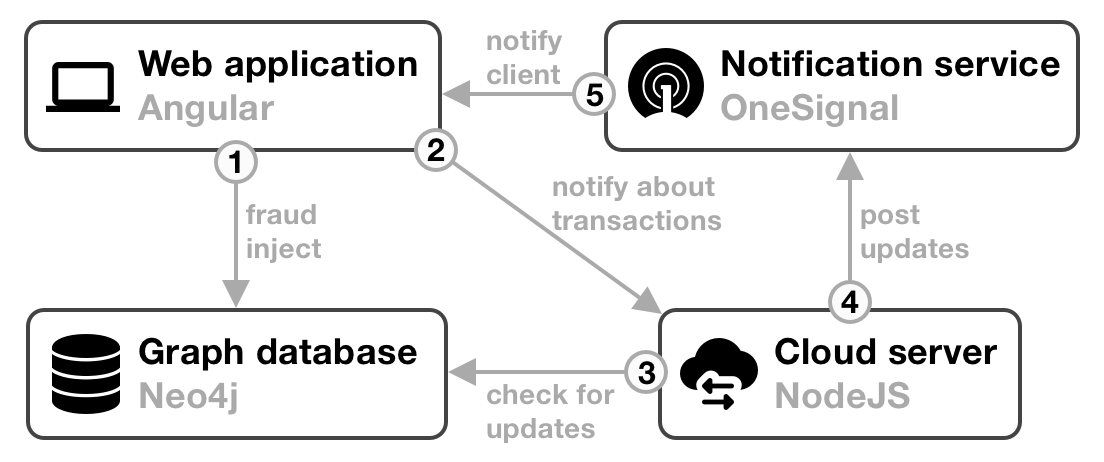
\includegraphics[width=0.7\textwidth]{figures/software_stack.png}
  \caption{Dynamic monitoring platform software stack} 
  \label{fig:software_stack}
\end{figure}

\subsection{Stored Procedure Library: Neo4j APOC}

APOC is a user-defined procedure and functions bundle for the Neo4j database.
It was written in Java and can be easily called within Cypher queries.
The library consists of more than 450 procedures, including data migration, integration, and mathematical procedure blocks.

In our use case, we used background operations from the APOC library to execute delta queries on each new transaction commits\footnote{\url{https://neo4j.com/docs/labs/apoc/4.0/background-operations/}}.
Triggers can be configured to be executed in synchronous/asynchronous behavior and before/after the transaction.

Delta queries for our three fraud cases are designed to be triggered at a new relationship to create a transaction.
The query will start to compute the required parameters starting with connected nodes of the relationship and assign the required flag for them.

\paragraph{``Smurfing'' delta query procedure}

For example, we have an initial graph like in the upper part of \autoref{fig:smurfing_incoming_transaction}, and none of the \texttt{User} nodes are flaged as \textit{smurfingSuspicious}.
If we add new relationship connections between the sender and receiver through a new middleman account, our registered trigger procedure will check them against the fraudulent pattern matching.

\begin{figure}[!ht]
  \centering
  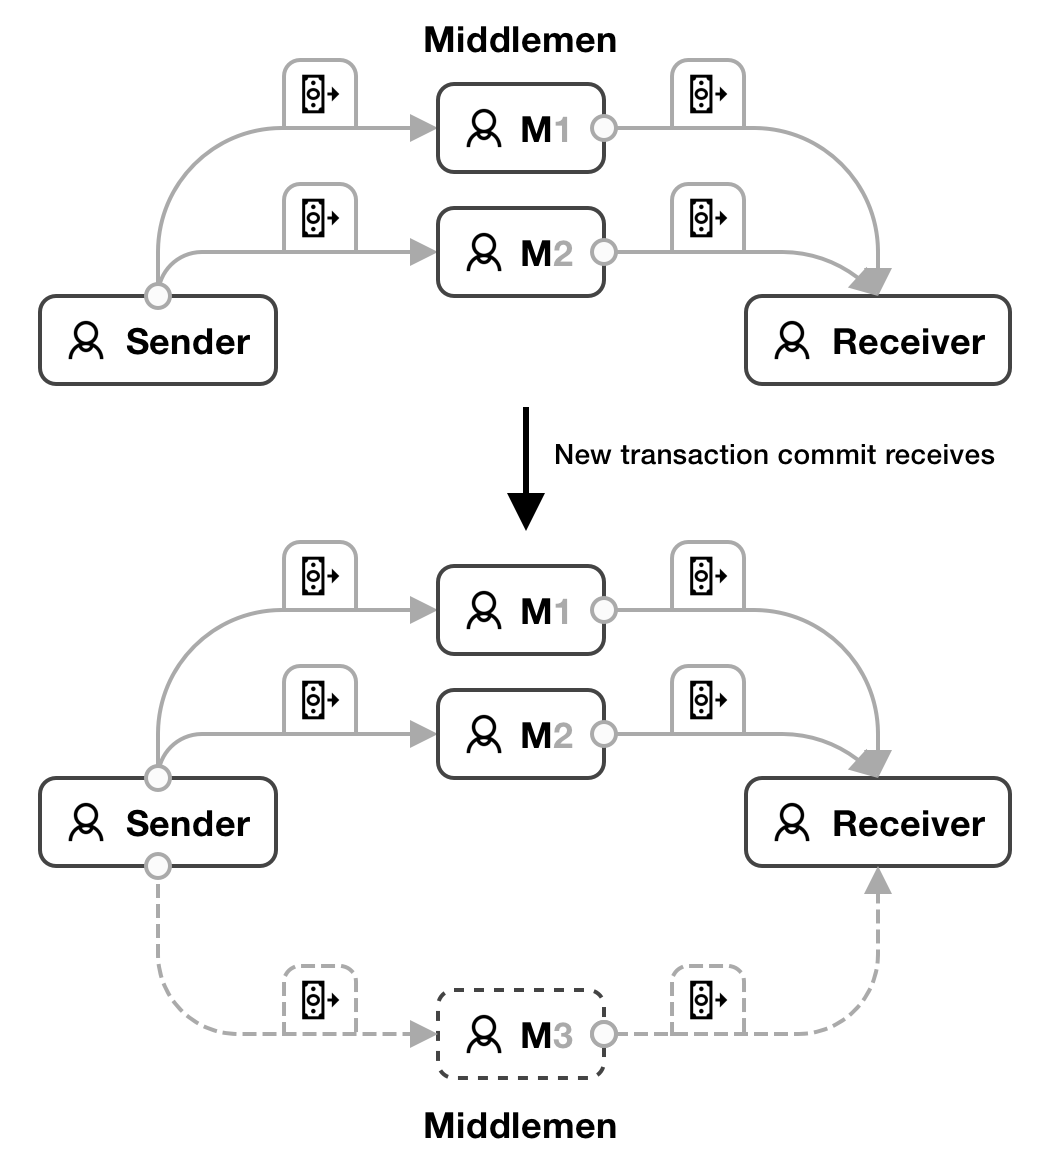
\includegraphics[scale=0.3]{figures/smurfing_incoming_transaction.png}
  \caption{A graph after commiting new relationship transactions}
  \label{fig:smurfing_incoming_transaction}
\end{figure}

The procedure in \autoref{lst:smurfing_delta_query} will trigger the smurfing fraud detection query just before the new relationship creates a transaction.
In our delta query, the destination node is taken from the created relationship, then the smurfing fraud pattern matching is applied to it.
Here we update the database incrementally at each transaction and mark the fraudulent users to be queried faster in the future.

\lstset{language=cypher,
	literate=*
	{qqq}{'}{1}
}
\begin{lstlisting}[language=Cypher,frame=single,caption={Smurfing delta query procedure},label={lst:smurfing_delta_query}]
CALL apoc.trigger.add('detect_smurfing',
  qqqUNWIND $createdRelationships AS tr
  WITH endNode(tr) AS receiver
  MATCH (sender:User)-[:SENT_TO]->(pm:User)-[:SENT_TO]->(receiver)
  WITH sender, receiver, count(pm) AS pms
  WHERE pms >= 3
  SET receiver.smurfingSuspicious = trueqqq,
  {phase:'before'}
)
\end{lstlisting}

In our work, we got an output graph snapshot after injecting a series of fraudulent transactions with a suspicious receiver user entry named \textit{Sydney Snider} (\autoref{fig:smurfing_suspicious_node}).

\begin{figure}[!ht]
  \centering
  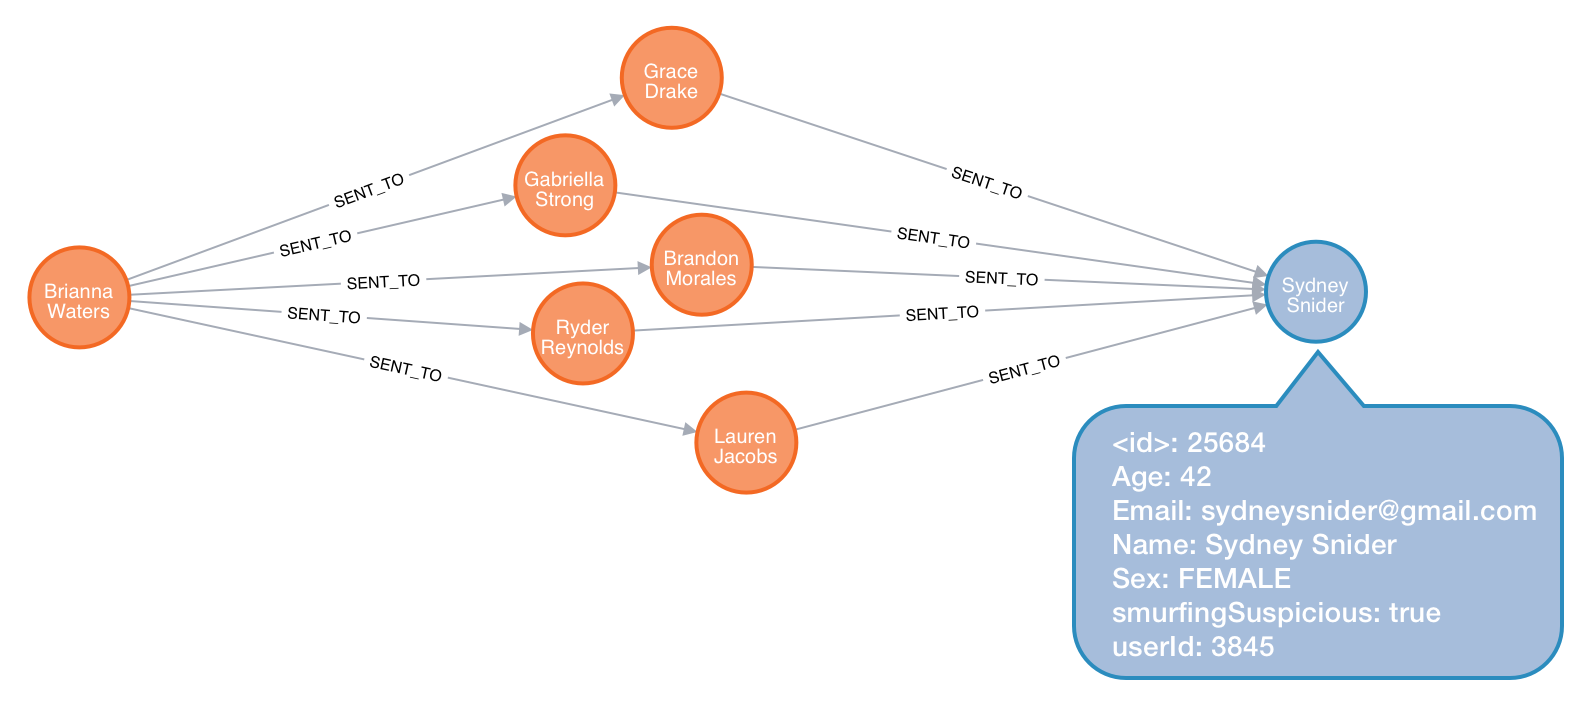
\includegraphics[width=\textwidth]{figures/smurfing_suspicious_node.png}
  \caption{A graph snapshot after a fradulent transaction commit} 
  \label{fig:smurfing_suspicious_node}
\end{figure}

\paragraph{``Money laundering'' delta query procedure}

In the money laundering scenario, both connected nodes of the newly created relationship are used in the delta query.
We are looking for the other three middlemen participation in our graph by pattern matching.
If the fraud case is detected for the destination node, we mark the original sender and destination nodes as \texttt{moneyLaunderingSuspicious}.

\lstset{language=cypher,
	literate=*
	{qqq}{'}{1}
}
\begin{lstlisting}[language=Cypher,frame=single,caption={Money laundering delta query procedure},label={lst:money_laundering_delta_query}]
CALL apoc.trigger.add('detect_money_laundering',
  qqqUNWIND $createdRelationships AS tr
  WITH tr
  WITH startNode(tr) as m4, endNode(tr) AS receiver
  WITH receiver, m4
  MATCH (sender:User)-[:SENT_TO]->(m1:User)-[:SENT_TO]->(m2:User)-[:SENT_TO]->(m3:User)-[:SENT_TO]->(m4)-[:SENT_TO]->(receiver)-[c:CONNECTED_TO]-(sender)
  SET sender.moneyLaunderingSuspicious = true
  SET receiver.moneyLaunderingSuspicious = trueqqq,
  {phase:'before'}
)
\end{lstlisting}
   
\paragraph{``Biased reviews'' delta query procedure}

As previous procedures, the delta query is executed before the relationship creates the transaction.
In this case, a new review relationship is detected, and connected \texttt{User} and \texttt{Good} nodes are taken for the following evaluations.
First, the merchant node is obtained through the ownership relationship with the referenced good node.
Then we match the original biased reviews pattern with a constrained user and merchant nodes.
The constrained nodes simplify the matching calculation significantly and allow us to implement IVM effectively.
If users and merchants are matched as biased reviews fraud actors, they will be marked as \texttt{biasedReviewsSuspicious}.

\lstset{language=cypher,
	literate=*
	{qqq}{'}{1}
}
\begin{lstlisting}[language=Cypher,frame=single,caption={Biased reviews delta query procedure},label={lst:biased_reviews_delta_query}]
CALL apoc.trigger.add('detect_biased_reviews',
  qqqUNWIND $createdRelationships AS rev
  WITH rev
  WITH startNode(rev) as sender, endNode(rev) AS good
  WITH good
  MATCH (good)-[:OWNED_BY]->(m:Merchant)
  WITH m
  MATCH (u:User)-[r:REVIEWED_TO]->(g:Good)-[o:OWNED_BY]->(m)
  WITH u, m, collect(r) as reviews, collect(g) as goods
      WHERE size(reviews) >= 4
  UNWIND reviews as revList
  WITH avg(toInteger(revList.Rating)) as avgRating, u, m, goods, reviews
      WHERE avgRating >= 4
  SET m.biasedReviewsSuspicious = true
  SET u.biasedReviewsSuspicious = trueqqq,
  {phase:'before'}
)
\end{lstlisting}

\subsection{Cloud server: Node JS}

A cloud server is configured in the Node JS runtime environment to maintain the periodic remote monitoring over graph database.
The primary role of the server is checking the graph database for fraud case updates.
In our setup at the second step in \autoref{fig:software_stack}, the server is notified with HTTP post request after each transaction commit.
The cloud server also sends query commands to graph database over HTTP post request payload and gets a response asynchronously.
Cypher queries for each fraud case are stored in the server methods and focused on the matching fraud actors' number.
To deliver the newly detected fraud actors, we store each query results in the server's runtime memory.
If the incoming fraud case result differs from the previous one, we call push notification service provider over the network (step 4 in \autoref{fig:software_stack}). 

\subsection{Push notification provider: OneSignal}

The OneSignal web service is used as a notification provider for client web applications about the update notifications in our software stack.
First, we created a project in OneSignal web application and got our project credentials.
There are two SDKs for both, and client applications and integration steps are documented well.
On the client-side, a button appears at the first startup for notification service subscriptions. If the user accepts, it will disappear for the next sessions.
OneSignal supports most of the modern browsers, even in mobile versions.
User will get the notification even web application is closed.
We set up the service provider module with our project credentials from the server-side, and then we can quickly call it in our environment.
As mentioned above, the cloud server will call the notification service if new fraud actors are detected, then OneSignal will handle the rest of the notification delivery process (step 5 in \autoref{fig:software_stack}).

\subsection{Web application: Angular}

The front-end side of the monitoring system is developed in one of the modern and popular JavaScript frameworks, Angular.
Angular is designed to deliver web and mobile applications with one codebase.
The framework gives high customizable templating opportunities and converts them into native optimized JavaScript code in the production.
Angular consists of 3 general building blocks, modules, components, and services.
In our web demo, we used a few components to show interactive views, one module to combine the dashboard components, and two services to handle network requests.
In the dashboard page (\autoref{fig:web_demo_smurfing}), we have a collapsable toolbar on the left panel and graph visualizer on the right.

The visualization component is engineered with using D3 JavaScript library\footnote{\url{https://d3js.org/}}.
The library offers a wide variety of SVG (Scalable Vector Graphics) animations and visualization tools.
The data source is obtained from the graph database over the network and parsed into the corresponding \textit{Node} and \textit{Link} elements of the library.
The graph is always in floating motion and handles medium-sized datasets (graphs of a few hundred nodes) efficiently.

By clicking the \textbf{Inject fraudulent transactions} button, our service will generate fraud relationships for our graph setup and commits them to the database over the network (step 1 in \autoref{fig:software_stack}).
The fradulent relationships generation algorithm is a converted version of our Java based data generator (discussed in \textbf{\nameref{sec:syntetic_data_generator}}) in Typescript language.
During the fraud generation, the nodes are selected based on predefined ID range; for example, \texttt{User} nodes are defined from 0 to 20k, \texttt{Good} nodes from 20k to 40k, etc. The varieties differ due to the scale of the datasets. 
After picking the required node ID, the fraud pattern query is build using relationship assignment commands in Cypher language, then committed to the Neo4j database.

\begin{figure}[!ht]
  \centering
  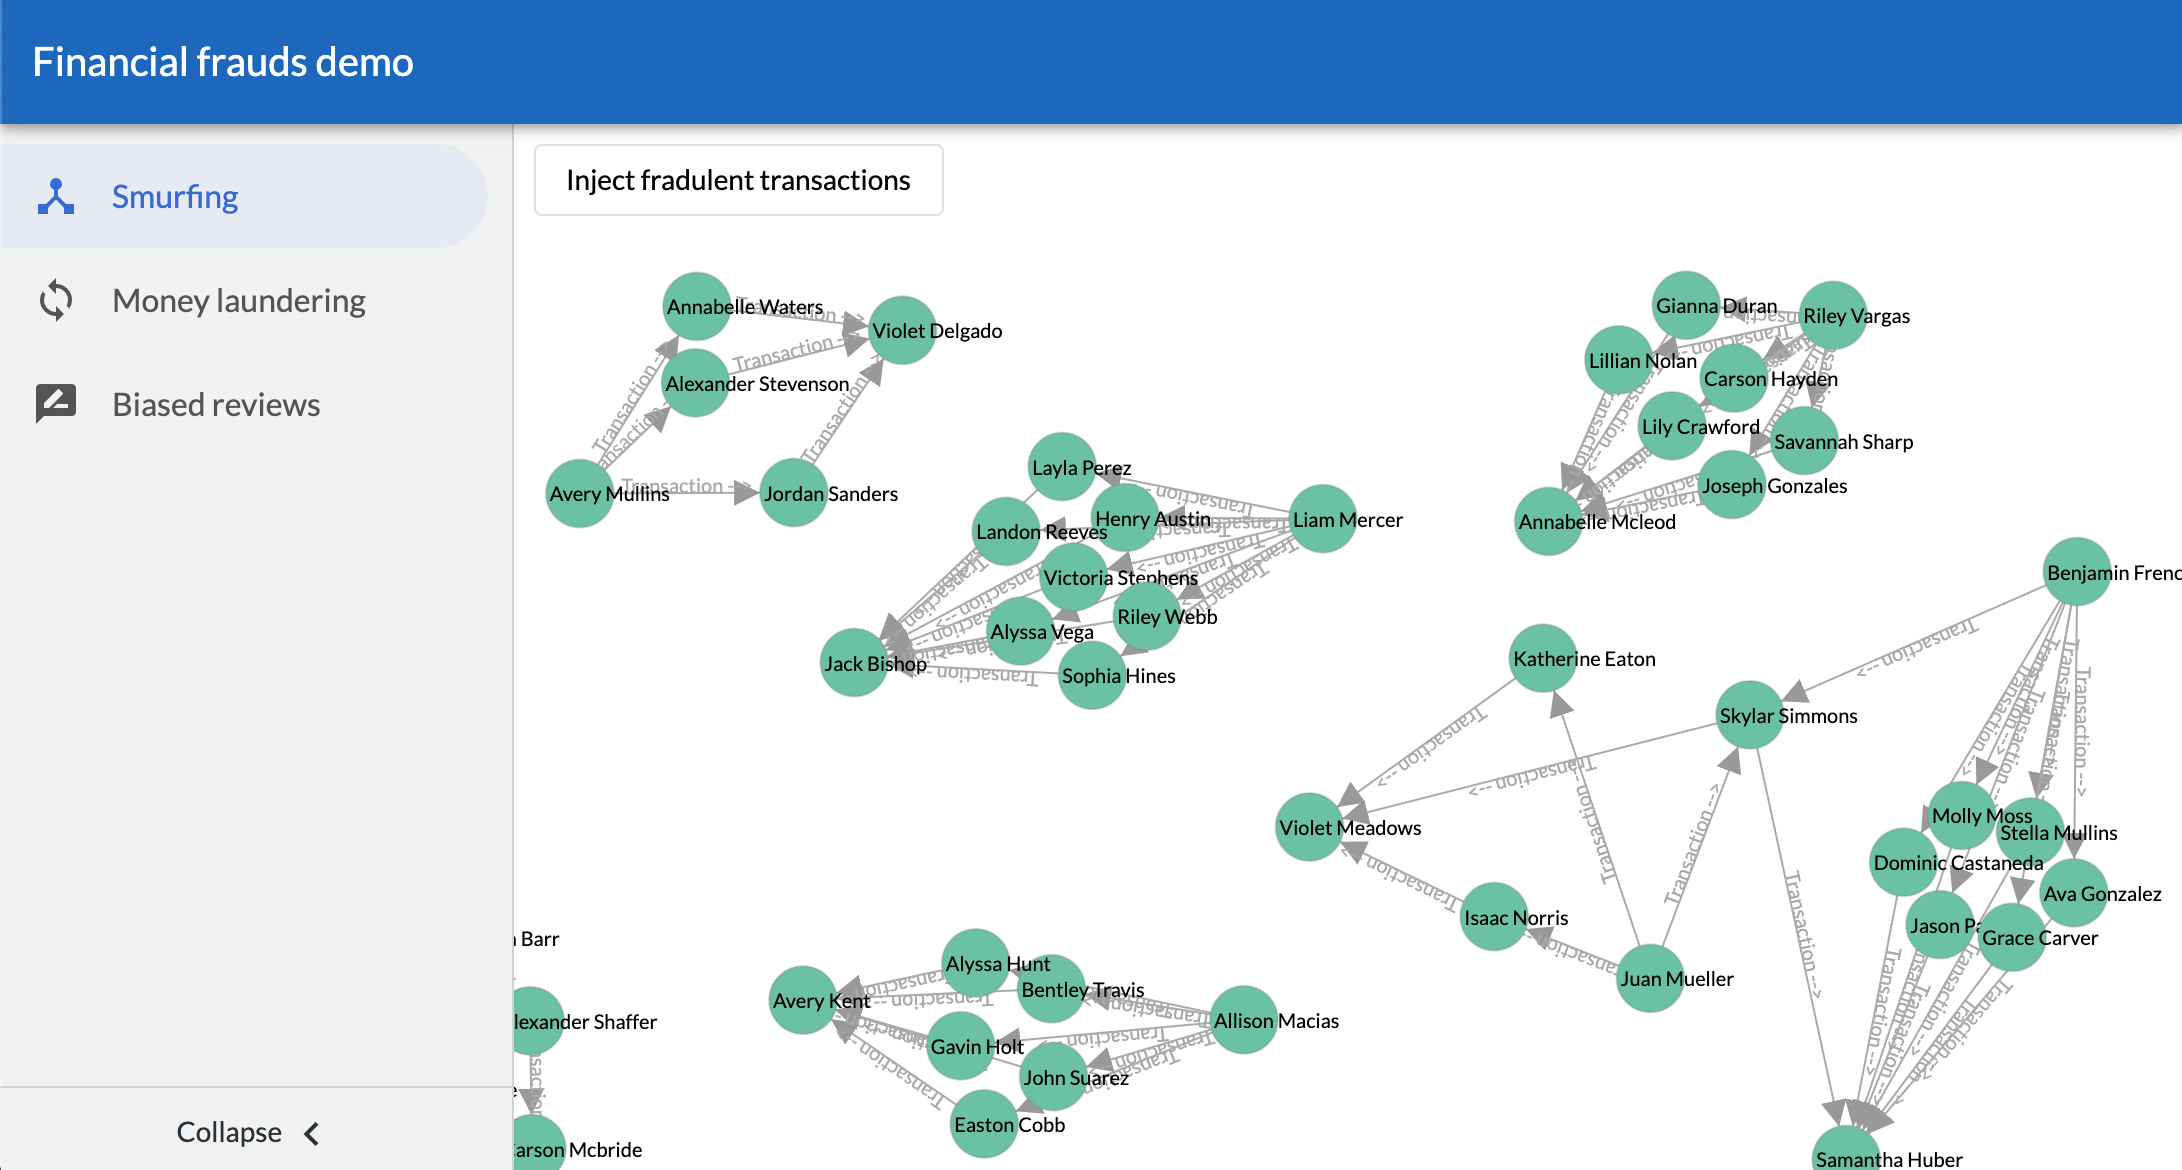
\includegraphics[width=\textwidth]{figures/web_demo_smurfing.png}
  \caption{Web demo -- smurfing fraud monitoring} 
  \label{fig:web_demo_smurfing}
\end{figure}

%----------------------------------------------------------------------------
\section{Benchmark}
%----------------------------------------------------------------------------

To examine the performance of dynamic implementation over the static one, we benchmarked the query execution times.
The execution time is measured with millisecond precision.
The simplified version of original queries is used in static measurements; the only number of fraudulent actors are returned.
The reduction in the response body decreased execution time of static queries.
The execution time covers the whole relationship insert processes followed by individual delta queries in the dynamic implementation.
Despite the accumulated query commands, dynamic queries are completed faster than static ones in most cases.
The benchmark was executed on a MacBook Pro 2015 laptop with an Intel Core i7 CPU and 16 GB RAM, using Java 11.0.6 JVM.

\paragraph{Small dataset} The queries are successfully completed in the small dataset (\autoref{fig:benchmark_small}).
Dynamic queries are performed 10 and 100 times faster than static alternatives, respectively, in smurfing and money laundering cases.
In the case of the biased reviews, the static implementation is slightly faster than the dynamic one.
If we consider the summed execution time in dynamic implementation, one of the relationship creation queries is completed 8--10 times less. 

\paragraph{Large dataset} Not all the queries are completed successfully in large dataset experiments (\autoref{fig:benchmark_large}).
In the smurfing one, we gained more than 180 times faster performance. 
As we failed to run a money-laundering query in the large dataset before (\autoref{sec:static_benchmark}), the dynamic version is also failed in experiments (as the initial evaluation did not complete within the timeout).
Compared with a small dataset, we got faster incremental query execution than the static implementation in a large dataset of biased reviews.
The performance gain in the biased reviews was $6\times$.

\begin{figure}[!ht]
  \centering
  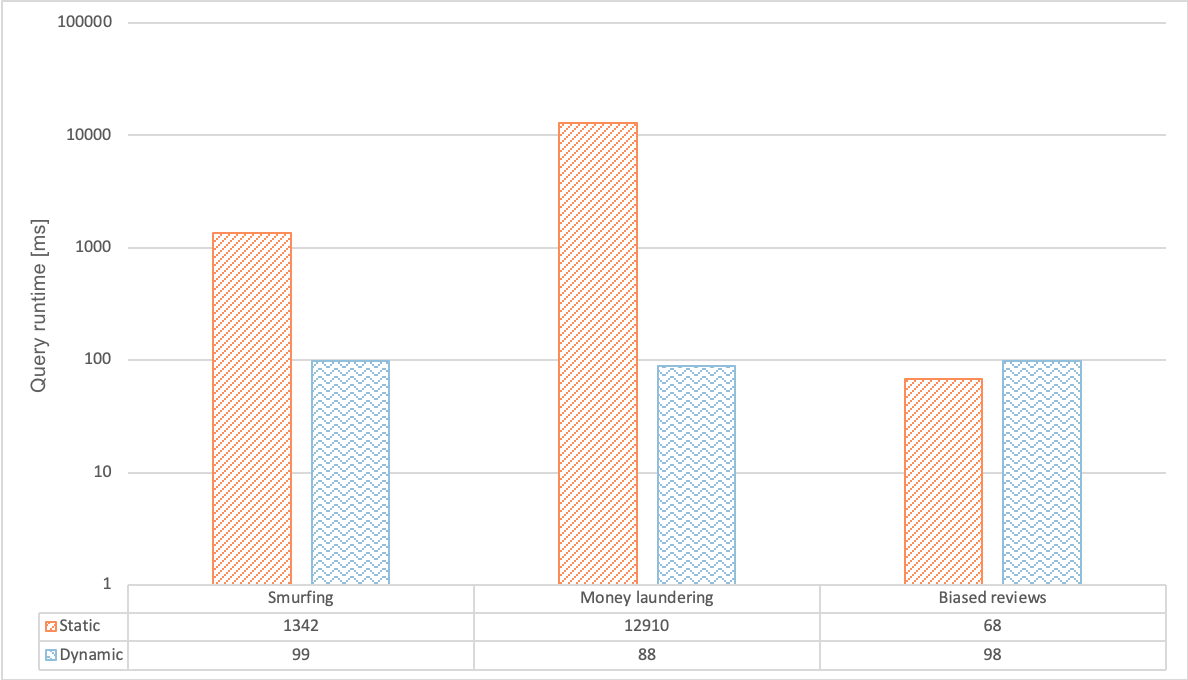
\includegraphics[width=\textwidth]{figures/dynamic_benchmark_plot_small.png}
  \caption{Small dataset dynamic implementation benchmark} 
  \label{fig:benchmark_small}
\end{figure}

\begin{figure}[!ht]
  \centering
  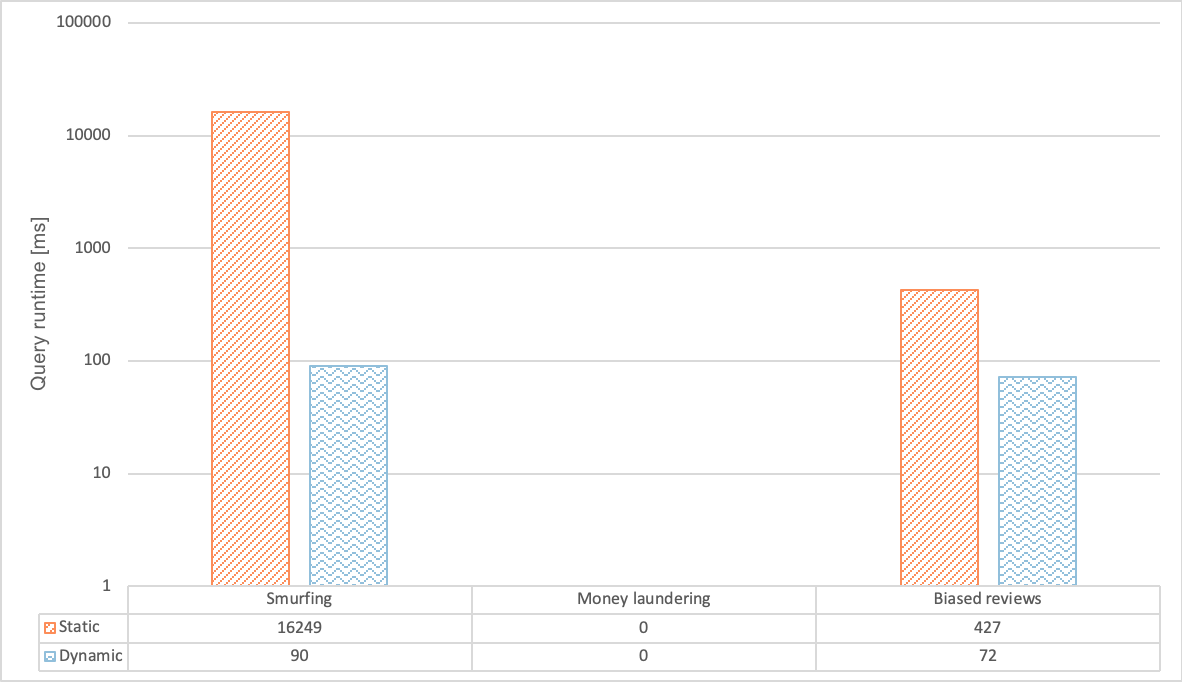
\includegraphics[width=\textwidth]{figures/dynamic_benchmark_plot_large.png}
  \caption{Large dataset dynamic implementation benchmark} 
  \label{fig:benchmark_large}
\end{figure}

%----------------------------------------------------------------------------
\section{Analysis}
%----------------------------------------------------------------------------

We got promising results during the experiments with incremental view maintenance implementation, a performance gain of 5--140 times in the small dataset and 6--180 times in the large dataset.
Based on these experiments, incremental view maintenance is recommended for getting faster query performance.
IVM can introduce the additional data in the database, which will increase the memory usage.
However, the extra memory usage is a worthy tradeoff due to the significant speedups in computation performance.

In the default graph setup, we faced slower benchmarks in the dynamic implementation part.
This behavior was unexpected; in theory, limited range pattern matching should not take much time.
First, data types are optimized with converting string IDs to integer types and applied ID indexing over nodes.
The performance was improved slightly and still not sufficient for real-world applications.
Second, we optimize the query itself; by intuition, the performance of the query is dominated by the lookup command.
The initial pattern matching command \autoref{lst:not_optimized_pattern} was querying the whole database, which is opposite to our goal. 
The problem was fixed by using the \texttt{startNode} and \texttt{endNode} methods (line 3 in \autoref{lst:snippet_start_end_nodes}).
This way, instead of evaluating another global pattern matching, the connected nodes of created relationships can be directly referenced in trigger procedures.

\begin{lstlisting}[language=Cypher,frame=single,caption={Unoptimized pattern matching},label={lst:not_optimized_pattern}]
UNWIND $createdRelationships AS tr
MATCH (:User)-[tr]->(receiver:User)
WITH startNode(tr) as m4, endNode(tr) AS receiver
\end{lstlisting}

\begin{lstlisting}[language=Cypher,frame=single,caption={A snippet of the optimized query with \texttt{startNode} and \texttt{endNode} methods},label={lst:snippet_start_end_nodes}]
UNWIND $createdRelationships AS tr
WITH startNode(tr) as m4, endNode(tr) AS receiverqqq
\end{lstlisting}
